\documentclass[../../main.tex]{subfiles}

% ベン図の共通設定
\newcommand{\VennFrame}{%
  \draw[thick] (-2.2,-3.9) rectangle (4.2,2.1);
  \node[anchor=north east] at (4.1,2.0) {$U$};
  \draw[thick] (0,0)     circle (1.6);
  \draw[thick] (2,0)     circle (1.6);
  \draw[thick] (1,-1.7)  circle (1.6);
  \node at (-1.3,1.55) {$A$};
  \node at ( 3.3,1.55) {$B$};
  \node at ( 1.0,-3.55) {$C$};
}

\begin{document}

{\bf [解]}
全世帯を100（\%）とし，ベン図の8つの領域の割合を次のようにおく．

\begin{center}
  \begin{figure}[htb]
    \centering
    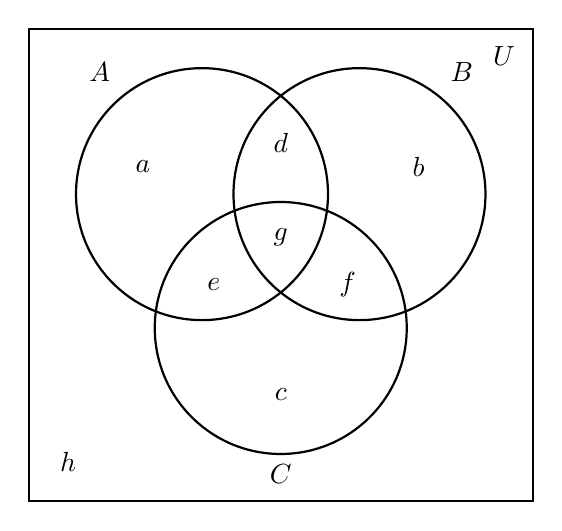
\begin{tikzpicture}
      \VennFrame
      \node at (-0.75, 0.35) {$a$};   % A のみ
      \node at ( 2.75, 0.35) {$b$};   % B のみ
      \node at ( 1.0, -2.55) {$c$};   % C のみ
      \node at ( 1.0,  0.65) {$d$};   % A∩B のみ
      \node at ( 0.15,-1.15) {$e$};   % A∩C のみ
      \node at ( 1.85,-1.15) {$f$};   % B∩C のみ
      \node at ( 1.0, -0.55) {$g$};   % A∩B∩C
      \node at (-1.7, -3.4)  {$h$};   % どれでもない
    \end{tikzpicture}
  \end{figure}
\end{center}

\begin{itemize}
  \item[] $a$：$A$のみ，\quad $b$：$B$のみ，\quad $c$：$C$のみ，\quad $d$：$A$と$B$のみ，
  \item[] $e$：$A$と$C$のみ，\quad $f$：$B$と$C$のみ，\quad $g$：3種類すべて，\quad $h$：どれも購読していない
\end{itemize}

題意の条件を図の領域で読みかえると以下のようになる．
\begin{align}
  &\text{$C$だけ}                 & c &= 3 \label{eq:1}\\
  &\text{$B$，$C$の両方}          & f+g &= 21 \label{eq:2}\\
  &\text{$B$}                     & b+d+f+g &= 46 \label{eq:3}\\
  &\text{$A$}                     & a+d+e+g &= 69 \label{eq:4}\\
  &\text{$A\cup C$ の外側}        & b+h &= 100-88 = 12 \label{eq:5}\\
  &\text{$B\cup C$ の外側}        & a+h &= 100-50 = 50 \label{eq:6}\\
  &\text{1種類だけ}               & a+b+c &= 61 \label{eq:7}
\end{align}

求める値は
\begin{enumerate}
  \item $A$だけを購読しているものの割合: $a$
  \item $B$だけを購読しているものの割合: $b$
  \item $A$，$B$，$C$すべてを購読しているものの割合: $g$
  \item $A$，$B$，$C$のどれも購読していないものの割合: $h$
\end{enumerate}
であるから順番に検討する．

まずは$a,b,h$について考える．\cref{eq:1}を\cref{eq:7}に代入して
\begin{align}
  a+b = 61-c = 61-3 = 58 \label{eq:8}
\end{align}
である．\cref{eq:5,eq:6}を辺々たすと
\begin{align}
  a+b+2h=62
\end{align}
だから，\cref{eq:8}を代入すると
\begin{align}
  2h &= 62 - (a+b) = 62 - 58 = 4 \\
  \therefore
  h &= 2 \label{eq:9}
\end{align}
である．これを\cref{eq:5,eq:6}に代入して
\begin{align}
  \begin{cases}
    a = 50 - h = 48 \\
    b = 12 - h = 10
  \end{cases} \label{eq:10}
\end{align}
である．

次に$d$を考えると，\cref{eq:2,eq:3}を辺々引いて
\begin{align}
  b+d=25
\end{align}
だから，\cref{eq:10}より
\begin{align}
  d = 25 - b = 25 - 10 = 15 \label{eq:11}
\end{align}
である．

次に$e,f,g$を考える．
まず全体が$100$になることから
\begin{align}
  a+b+c+d+e+f+g+h=100 \label{eq:12}
\end{align}
である．ここに\cref{eq:1,eq:8,eq:9,eq10,eq:11}を代入して
\begin{align}
  e+f+g = 100 - (48+10+3+15+2) = 22 \label{eq:12}
\end{align}
である．\cref{eq:2}を代入して
\begin{align}
  e = 22 - (f+g) = 22 - 21 = 1 \label{eq:13}
\end{align}
であり，よって\cref{eq:4}に代入して
\begin{align}
  g = 69 - (a+d+e) = 69 - (48+15+1) = 5 \label{eq:14}
\end{align}
である．よって\cref{eq:2}に代入して
\begin{align}
  f = 21 - g = 21 - 5 = 16 \label{eq:15}
\end{align}
である．以上の値をベン図に反映すると以下のようになる．

\begin{figure}[htb]
  \begin{center}
    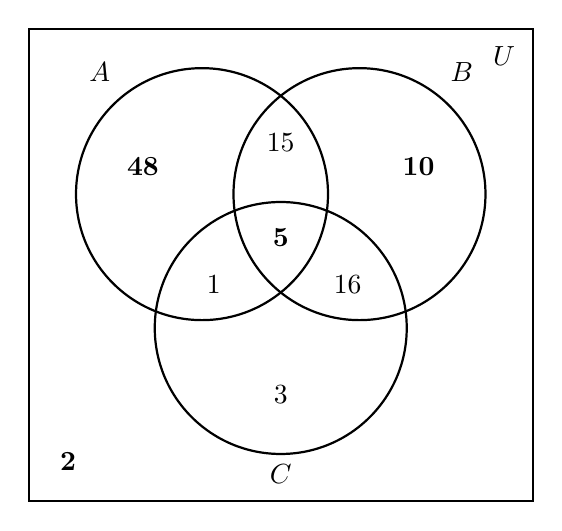
\begin{tikzpicture}
      \VennFrame
      \node at (-0.75, 0.35) {\textbf{48}};
      \node at ( 2.75, 0.35) {\textbf{10}};
      \node at ( 1.0, -2.55) {3};
      \node at ( 1.0,  0.65) {15};
      \node at ( 0.15,-1.15) {1};
      \node at ( 1.85,-1.15) {16};
      \node at ( 1.0, -0.55) {\textbf{5}};
      \node at (-1.7, -3.4)  {\textbf{2}};
    \end{tikzpicture}
    \caption{値を埋めたベン図}
  \end{center}
\end{figure}

求める答えは以下のようになる．
\begin{enumerate}
  \item $A$だけを購読しているもの：\textbf{48\%}
  \item $B$だけを購読しているもの：\textbf{10\%}
  \item $A$，$B$，$C$すべてを購読しているもの：\textbf{5\%}
  \item $A$，$B$，$C$のどれも購読していないもの：\textbf{2\%}
\end{enumerate}

\end{document}
